\section{System Overview}\label{sec:systemoverview}
In this section we give a short overview of the group recommendation system which is depicted in Figure \ref{fig:composition}. Each of the stages will be outlined with a short description. 

\paragraph{Individual Recommendation} We make individual recommendations for every user. The recommendation methods used in this step is interchangeable and can be selected to fit the data and purpose of the recommendation. The only condition for the recommender is that it finds a complete list of recommendations of the users in a group. In Section \ref{sec:individualrecommender} the recommender we use is further elaborated on.

\paragraph{Groups} In the groups stage we generated a list of groups for testing purposes. These groups consist of user id's and were generated at random but it is ensured that the same user only appears once in each group. The specific setup of the groups is described in Section \ref{sec:groupgeneration}.

\paragraph{Group Recommendation} The group recommendation part consists of two stages, namely preprocessing and rank aggregation.
\begin{itemize}
\item Preprocessing is needed to find the individual recommendations belonging to the users in a certain group and format them for the rank aggregation.
\item Rank aggregation combines the individual recommendations into a list of size $k$ which should represent the groups preferences.
\end{itemize}
A more detailed description of the stages in group recommendation can be found in Section \ref{sec:grouprecommendation}.
%\paragraph{Preprocessing} Before being able to aggregate the ratings preprocessing is needed. The preprocessing step takes a group as input and is concerned with finding the $k$ highest rated items for each of the users in the group. The items are arranged in a ranked lists with the highest rated item first and descending. The lists are stored in an array. A more detailed explanation of the preprocessing can be found in the introduction to Section \ref{sec:aggregations}.

%\paragraph{Aggregation} In the aggregation stage a selection of different aggregation methods was implemented and was interchangeable with each other. All the methods took the array of lists, which was supplied from the preprocessing stage, as input. The output of the aggregations is the group recommendation in the form of a ranked list of size $k$. In the subsections of Section \ref{sec:aggregations} are a description of the aggregation methods. 

\paragraph{Evaluation} The last stage is evaluation. In this stage several tests and measurements are performed. The setup and results of this stage is shown in Section \ref{sec:evaluation}.


%As we are going to aggregate recommendations we implemented a group recommender system with the steps shown in Figure \ref{fig:composition}. A dataset will provide for us to make some individual recommendations for users arranged into groups for later testing. The next part of the group recommender is the aggregation half, which is the focus of the paper. Using the output of the first part of the system, we will be trying several different aggregation approaches. The results of these are the group recommendations to be evaluated.
%As we take the aspect of aggregating recommendations the group recommendation system will consist of two parts namely an individual recommender and an aggregation method. \note{need some extension and probably an illustration}
\begin{figure}[t!]
\centering
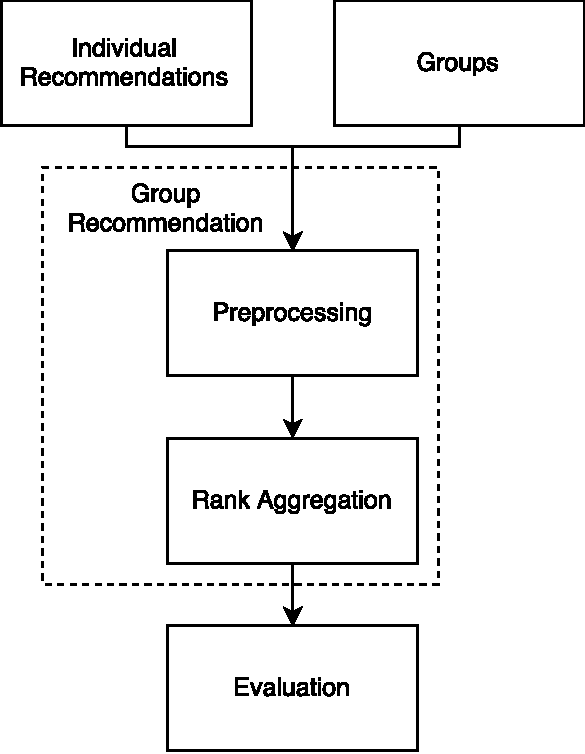
\includegraphics[scale=.4]{graphics/composition}
\caption{Stages of the group recommender system}\label{fig:composition}
\end{figure}